
\subsection*{1.}

\begin{center}
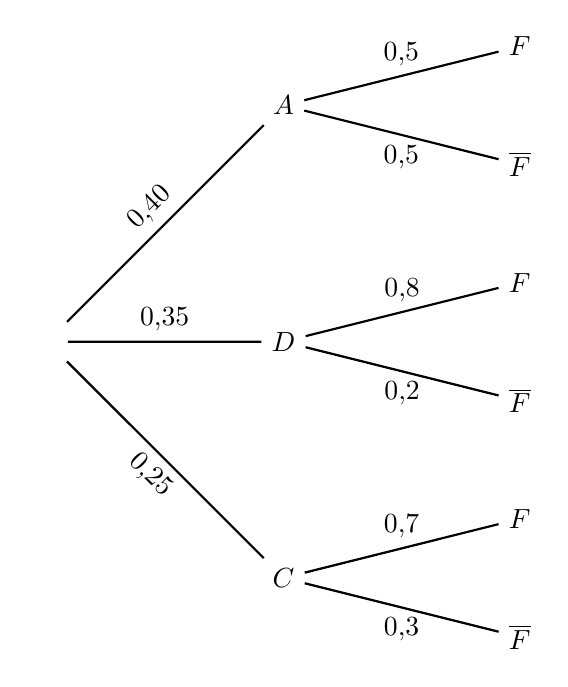
\begin{tikzpicture}[thick, scale=1.5] %{,}
\node (P_-1_0) at (-2,-2.5) {$\phantom{A}$};
\node (P_0_0) at (0,-0.5) {$A$};
\draw (P_-1_0) -- (P_0_0) node[midway, above,sloped] {$0{,}40$};
\node (P_1_0) at (2,-0) {$F$};
\draw (P_0_0) -- (P_1_0) node[midway, above] {$0{,}5$};
\node (P_1_1) at (2,-1) {$\overline{F}$};
\draw (P_0_0) -- (P_1_1) node[midway, below] {$0{,}5$};
\node (P_0_2) at (0,-2.5) {$D$};
\draw (P_-1_0) -- (P_0_2) node[midway, above] {$0{,}35$};
\node (P_1_2) at (2,-2) {$F$};
\draw (P_0_2) -- (P_1_2) node[midway, above] {$0{,}8$};
\node (P_1_3) at (2,-3) {$\overline{F}$};
\draw (P_0_2) -- (P_1_3) node[midway, below] {$0{,}2$};
\node (P_0_4) at (0,-4.5) {$C$};
\draw (P_-1_0) -- (P_0_4) node[midway, below,sloped] {$0{,}25$};
\node (P_1_4) at (2,-4) {$F$};
\draw (P_0_4) -- (P_1_4) node[midway, above] {$0{,}7$};
\node (P_1_5) at (2,-5) {$\overline{F}$};
\draw (P_0_4) -- (P_1_5) node[midway, below] {$0{,}3$};
\end{tikzpicture}
\end{center}

\subsection*{2.}

On a :
\[
p(A \cap F) = p(A) \times p_A(F) = 0{,}4 \times 0{,}5 = 0{,}2,
\]
\[
p(D \cap F) = p(D) \times p_D(F) = 0{,}35 \times 0{,}8 = 0{,}28,
\]
\[
p(C \cap F) = p(C) \times p_C(F) = 0{,}25 \times 0{,}7 = 0{,}175.
\]
D'après la loi des probabilités totales :
\[
p(F) = p(A \cap F) + p(D \cap F) + p(C \cap F) = 0{,}2 + 0{,}28 + 0{,}175 = 0{,}655.
\]

\subsection*{3.}

\[
P_F(D) = \dfrac{P(F \cap D)}{P(F)} = \dfrac{P(D \cap F)}{P(F)} = \dfrac{0{,}28}{0{,}655} \approx 0{,}4274,
\]
soit environs \(0{,}427\) au millième près.


\subsection*{4.}

\paragraph{a.} \( X \) ne peut prendre que deux valeurs :

\begin{itemize}
  \item 18 avec une probabilité de \(0{,}655\) ;
  \item 10 avec une probabilité de \( 1 - 0{,}655 = 0{,}345 \).
\end{itemize}

\paragraph{b.} Le coût moyen par spectateur d'une sortie dans ce cinéma est égal à l'espérance mathématique de la variable \( X \), soit :
\[
E(X) = 18 \times 0{,}655 + 10 \times 0{,}345 = 15{,}24 \, (\text{€}).
\]

